\documentclass[12pt]{article}
\usepackage[utf8]{inputenc}
\usepackage[margin=0.85in]{geometry}
\usepackage{amsmath,amssymb,enumitem}
\usepackage[most]{tcolorbox}
\usepackage{pgfplots}
\pgfplotsset{compat=1.17}
\setlength{\parindent}{0pt}
\begin{document}

\begin{center}{\Large\textbf{Solving Quadratics by Factoring}}\\[2pt]{\small Algebra I \textbar\ Guided Notes --- we fill these in together}\end{center}
Name: \rule{5cm}{0.4pt}\hfill Date: \rule{3cm}{0.4pt}
\vspace{0.3cm}

\begin{tcolorbox}[colback=blue!3,colframe=blue!55!black,title=Vocabulary --- write the definition]
\textbf{Zero Product Property:}\\[4pt]
\rule{\linewidth}{0.4pt}\\[12pt]
\rule{\linewidth}{0.4pt}\\[16pt]
\textbf{Root (solution):}\\[4pt]
\rule{\linewidth}{0.4pt}\\[12pt]
\rule{\linewidth}{0.4pt}
\end{tcolorbox}
\vspace{0.2cm}

\begin{tcolorbox}[colback=gray!4,colframe=gray!55!black,title=We do together --- worked example]
\textbf{Solve:}\quad $x^{2}+5x+6=0$\\[12pt]
\textbf{Step 1.}\ Get one side equal to $0$.\hfill(already done)\\[18pt]
\textbf{Step 2.}\ Factor the left side.\qquad $x^{2}+5x+6=\big(\underline{\hspace{2.4cm}}\big)\big(\underline{\hspace{2.4cm}}\big)$\\[26pt]
\textbf{Step 3.}\ Zero Product Property --- set \emph{each} factor equal to $0$.\\[10pt]
\hspace*{2.5em}$\underline{\hspace{3.2cm}}=0$\hspace{2.2cm}$\underline{\hspace{3.2cm}}=0$\\[26pt]
\textbf{Step 4.}\ Solve each little equation.\qquad $x=\underline{\hspace{1.8cm}}$\hspace{1.6cm}$x=\underline{\hspace{1.8cm}}$
\end{tcolorbox}
\vspace{0.2cm}

\textbf{See it on the graph.}\ The solutions are exactly where the parabola crosses the $x$-axis.\\[4pt]
\begin{center}
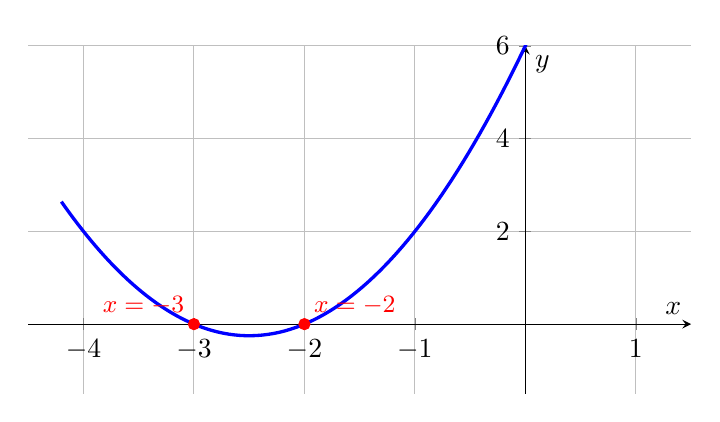
\begin{tikzpicture}
\begin{axis}[axis lines=middle,xlabel=$x$,ylabel=$y$,xmin=-4.5,xmax=1.5,ymin=-1.5,ymax=6,
  width=10cm,height=6cm,grid=both,xtick={-4,-3,-2,-1,0,1},ytick={2,4,6},samples=100]
\addplot[very thick,blue,domain=-4.2:0.8]{x^2+5*x+6};
\addplot[only marks,mark=*,red] coordinates {(-2,0)(-3,0)};
\node[above right,red,font=\small] at (axis cs:-2,0) {$x=-2$};
\node[above left,red,font=\small] at (axis cs:-3,0) {$x=-3$};
\end{axis}
\end{tikzpicture}
\end{center}
The graph crosses at $x=-2$ and $x=-3$ --- the same answers you found in Step 4.\\[10pt]

\textbf{You Try.}\ Solve $x^{2}-x-12=0$. Show every step, then name the two roots.\\[4cm]

\end{document}
